\section{Prototyp}
\subsection{Realisierung}
Für die Realisierung des Prototypen hat der Autor das Kennenlern-Angebot von AWS, ein einjähriges kostenloses Kontingent an Services und Produkten\cite{FreeTier2020}, gewählt. 

Nachdem der \emph{AWS Testaccount} erstellt war, mussten erste Schritte wie grundlegende Konfigurationen des Identity Access Management (IAM) gemacht und das Steuern von Spot Anfragen erlernt werden.

Weitere Schritte folgten. Die Realisierung des Prototypen wird in den folgenden Kapiteln beschrieben werden.

\begin{figure}[H]
	\centering
	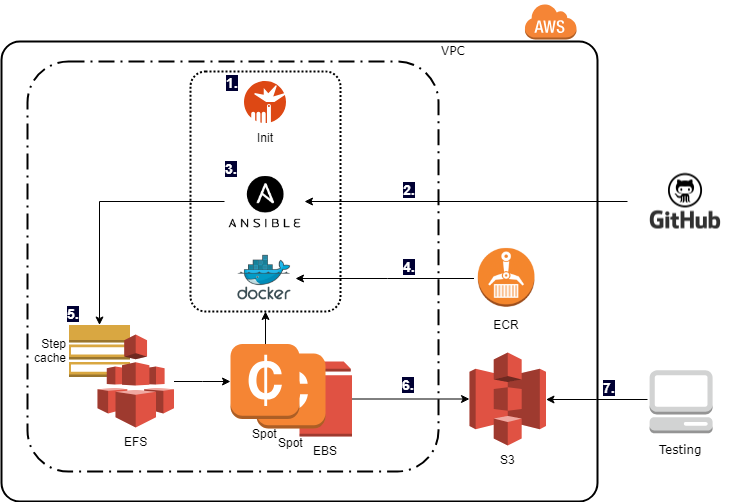
\includegraphics[width=.90\textwidth]{poc_zustand}
	\caption{Geodatenprozessierung mit SPOT Instanzen.}
	\label{fig:ist_zustand}
\end{figure}

\subsubsection{Der Publikationsvorgang als Code}
Mit der Entscheidung, die Spot Instanz via \emph{Cloud-Init}-Ansatz (Abb. \ref{fig:ist_zustand}, Nr. 1) mit Ansible zu Provisionieren\footnote{Und nicht via einem neuen AMI.}, lag es auf der Hand auch gleich Ansible für den Publikationsvorgang zu verwenden (Nr. 3).

Das Init-Skript wie auch die Ansible Deklarationen können \href{https://github.com/bfh-semesterarbeit/up-and-running-dataprocessing}{auf github.com/bfh-semesterarbeit} angeschaut werden.




\subsubsection{Handling der Interrupts}
Sämtliche Schritte werden via Ansible verwaltet und sobald ein Schritt erledigt wurde, hält Ansible dies auf dem gemounteten EFS Volumen in einer Textdatei fest.

Falls es zu einem Interrupt kommen sollte, wird von der Spot Flotte die nächste Instanz bereitgestellt und Ansible macht bei dem Schritt weiter, der zuletzt in der Textdatei festgehalten wurde (Abbildung \ref{fig:ist_zustand}, Nr. 5).


\subsection{Testen}

\paragraph{Testen der Datenstruktur}


\paragraph{Unerwartetes Herunterfahren}


\paragraph{Real Case Szenario}

Der komplette Rohdatensatz, alle Gebäude der Schweiz, wurde prozessiert. Das Resultat kann vorläufig\footnote{Bis am 1. November 2020} hier betrachtet werden:
\href{https://codepen.io/rebert/pen/ExKZmmE}{https://codepen.io/rebert/pen/ExKZmmE} Wobei nur die Gebäude vom S3 Testbucket kommen (Abb. \ref{fig:ist_zustand}, Nr. 7) 
